\chapter{Classification}
\label{chap-classification}

%%%%%%%%%%%%%%%%%%%%%%%%%%%%%%%%%%%%%%%%%%%%%%%%%%%%%%%%%%%%%%%%%%%%%%%%%%%%%
\section{Classification}

Classification is a machine learning problem seeking to map from
inputs $\R^d$ to outputs in an\anchorednote{unordered set.}{in contrast to a continuous real-valued
  output, as we saw for linear regression} \index{classification}
Examples of classification output sets could be $\{{\text apples}, {\text oranges}, {\text pears}\}$ if we're
trying to figure out what type of fruit we have, or
$\{{\text heart attack}, {\text no heart attack}\}$ if we're working in an emergency
room and trying to give the best medical care to a new patient.
We focus on an essential simple
case, {\em binary classification}, where we aim to find a mapping from $\R^d$ to
two outputs. \index{classification!binary classification}
While we should think of the outputs as not having an order, it's
often convenient to encode them as $\{-1, +1\}$.  As before, let the letter $h$ (for
hypothesis) represent a classifier, so the classification process
looks like:
$$ x \rightarrow \boxed{h} \rightarrow y \;\;.$$
%
% As with regression, real life rarely gives us vectors of real numbers;  the $x$ we really
% want to classify is often some rich visual, audio, or other physical data.
% In that case, we'll have to define a function $\varphi(x)$, whose
% domain is $\R^d$, where $\varphi$ represents 
% {\em features} of $x$, like a person's height or the amount of bass in
% a song, and then let the $h: \varphi(x) \rightarrow \{-1, +1\}$. 
% In much of the following, we'll omit explicit mention of $\varphi$ and
% assume that the $\ex{x}{i}$ are in $\R^d$, but you should always have
% in mind that some additional process was almost surely required to go
% from the actual input examples to their feature representation.
%
Like regression, classification is a {\em{supervised learning}} problem, in which we
are given a training data set of the form
\[ \data_n = \left\{\left(\ex{x}{1}, \ex{y}{1}\right), \dots, \left(\ex{x}{n},
  \ex{y}{n}\right)\right\} \;\;.\]
We will assume that each $\ex{x}{i}$ is a $d \times 1$ {\em column
    vector}. The intended use of this data is that, when given an input
$\ex{x}{i}$, the learned hypothesis should generate output
$\ex{y}{i}$.

What makes a classifier useful?  As in regression, we want it to work well on
% \anchorednote{{\em new}}{My favorite analogy is to problem sets.  We evaluate a
%   student's ability to {\em generalize} by putting questions on
%   the exam (test set) that were not on the homework (training set).}
new data, making good predictions on examples it hasn't seen.
But we don't know exactly what data this classifier might be tested on
when we use it in the real world. So, we have to {\em{assume}} a
connection between the training data and testing data; typically, they
are drawn independently from the same probability distribution.

In classification, we will often use 0-1 loss for evaluation
(as discussed in Section~\ref{sec-evaluation}). For that choice, we can
write the training error and the testing error.
In particular, given a training set $\data_n$ and a classifier $h$, we define the
  {\em{training error}} of $h$ to be
\begin{eqnarray*}
  \trainerr(h) = \frac{1}{n}\sum_{i = 1}^{n}\begin{cases} 1 &
              h(\ex{x}{i}) \ne \ex{y}{i} \\ 0 & \text{otherwise}\end{cases}
  \;\;.
\end{eqnarray*}

For now, we will try to find a classifier with small training error
(later, with some added criteria) and hope it {\em{generalizes well}}
to new data, and has a small {\em test error}
\begin{eqnarray*}
  \mathcal{E}(h) = \frac{1}{n'}\sum_{i = n + 1}^{n + n'}\begin{cases}
    1 & h(x^{(i)}) \ne y^{(i)} \\ 0 & \text{otherwise}\end{cases}
\end{eqnarray*}
on $n'$ new examples that were not used in the process of finding the
classifier.

% {\bf What is the role of hypothesis classes for classifiers?}
% A {\em hypothesis class} $\hclass$ is a set (finite or infinite) of
% possible classifiers, each of which represents a mapping from 
% $\R^d \rightarrow \{-1, +1\}$.

% A {\em learning algorithm} is a 
% procedure that takes a data set $\data_n$ as input and returns an
% element $h$ of $\hclass$;  it looks  like
% \begin{equation*}
%   \data_n \longrightarrow \boxed{\text{learning alg ($\hclass$)}} \longrightarrow h
% \end{equation*}

% We will find that the choice of $\hclass$ can have a big impact on the
% test error of the $h$ that results from this process.  One way to get
% $h$ that generalizes well is to restrict the size, or
% ``expressiveness'' of $\hclass$.
We begin by introducing
the hypothesis class of {\em linear classifiers}\index{linear classifier}
(Section~\ref{sec-linear_classifiers}) and then define
an optimization framework to learn {\em linear logistic
    classifiers} (Section~\ref{sec-lin_log_classifiers}).

% We then
% return to feature representation, in the context of classifiers
% (Section~\ref{sec-features_classifiers}).

%%%%%%%%%%%%%%%%%%%%%%%%%%%%%%%%%%%%%%%%%%%%%%%%%%%%%%%%%%%%%%%%%%%%%%%%%%%%%
\section{Linear classifiers}

\label{sec-linear_classifiers}

We start with the hypothesis class of {\em linear classifiers}.  They
are (relatively) easy to understand, simple in a mathematical sense,
powerful on their own, and the basis for many other more sophisticated
methods.  Following their definition, we present a simple
learning algorithm for classifiers.

%%%%%%%%%%%%%%%%%%%%%%%%%%%%%%%%%%%%%%%%
\subsection{Linear classifiers: definition}

A linear classifier in $d$ dimensions is
defined by a vector of parameters $\theta \in \R^d$ and scalar
$\theta_0 \in \R$.  So, the hypothesis class $\hclass$ of linear
classifiers in $d$ dimensions is parameterized by the {\em set} of all vectors in
$\R^{d+1}$.   We'll assume that $\theta$ is a $d \times 1$ column
vector.

Given particular values for $\theta$ and $\theta_0$, the classifier is
defined by
% {Let's be careful about dimensions.  We have assumed that $x$ and
%   $\theta$ are both $d \times 1$ column vectors.  So $\theta^T x$ is $1
% \times 1$, which in math (but not necessarily numpy) is the same as a
% scalar.} 
\begin{eqnarray*}
  h(x; \theta, \theta_0) = \text{sign}(\theta^T x + \theta_0)
  = \begin{cases} +1 & \text{if $\theta^Tx + \theta_0 > 0$} \\ -1 &
              \text{otherwise}\end{cases} \;\;.
\end{eqnarray*}
\index{linear classifier!hypothesis class}\index{sign function}Remember that we can think of $\theta, \theta_0$ as specifying a
$d$-dimensional hyperplane (compare the above with
Eq.~\ref{eq:linear_reg_hypothesis}).  But this time, rather than
being interested in that hyperplane's values at particular points $x$,
we will focus on the {\em separator} that it induces.  The separator
is the set of $x$ values such that $\theta^T x + \theta_0 = 0$.  This
is also a hyperplane, but in $d-1$ dimensions!\index{separator}
We can interpret $\theta$ as a
vector that is perpendicular to the separator.  (We will also say
that $\theta$ is {\em normal to} the separator.)

For example, in two dimensions ($d=2$) the separator has dimension 1,
which means it is a line, and
the two components of $\theta = [\theta_1, \theta_2]^T$ give the orientation
of the separator, as illustrated in the following example.

\subsection{Linear classifiers: examples}

%%%%%%%%%%%%%%%%%%%%

\begin{examplebox}{\bf Example:}
  Let $h$ be the linear classifier defined by $\theta = \protect\twodcol{1}{-1}, \theta_0 = 1$.

  \bigskip
  \noindent
  The diagram below shows the $\theta$ vector (in green) and the separator
  it defines:

  \begin{center}
    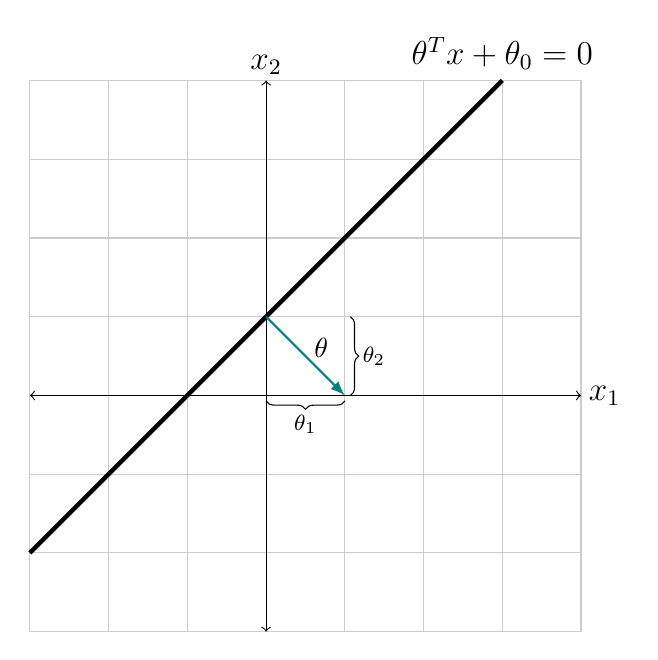
\begin{tikzpicture}
      \draw [thin, gray!40] (-3,-3) grid (4,4);
      \draw [<->] (-3,0) -- (4,0);
      \draw [<->] (0,-3) -- (0,4);

      \draw [ultra thick] (-3, -2) -- (3, 4)
      node [above] {\large$\theta^Tx + \theta_0 = 0$};

      \node [xshift=0em] at (4.3,0) {\large$x_1$};
      \node [xshift=0em] at (0,4.2) {\large$x_2$};

      % \draw [thick,teal,-latex] (0, 1) -- (0.9, 0.1)
      \draw [thick,teal,-latex] (0, 1) -- (1.0, 0.0)
      % node [black,below right] {$\theta$};
      node [black,midway, xshift=0.2cm,yshift=0.1cm] {$\theta$};

      \draw [decorate,decoration={brace,amplitude=3pt, mirror},xshift=2pt,yshift=0pt]
      (1,0) -- (1.0,1.0) node [black,midway,xshift=0.3cm]
      {\footnotesize $\theta_2$};

      \draw [decorate,decoration={brace,amplitude=3pt, mirror},xshift=0pt,yshift=-2pt]
      (0,0) -- (1.0,0.0) node [black,midway,yshift=-0.3cm]
      {\footnotesize $\theta_1$};
    \end{tikzpicture}

  \end{center}

  What is $\theta_0$?  We can solve for it by plugging a point
  on the line into the equation for the line.  It is often convenient to choose a point on one of the axes, e.g., in this case,
  $x=[0, 1]^T$, for which $\theta^T \left[ \begin{array}{c} 0 \\ 1 \end{array} \right] + \theta_0 = 0$, giving $\theta_0 = 1$.

\end{examplebox}

%%%%%%%%%%%%%%%%%%%%

In this example, the separator divides $\R^d$, the space our $\ex{x}{i}$ points live
in, into two half-spaces.  The one that is on the same side as the
normal vector is the {\em positive} half-space, and we classify all
points in that space as positive.  The half-space on the other side is
  {\em negative} and all points in it are classified as negative.

Note that we will call a separator a {\em linear separator}\index{separator!linear separator} of a data set
if all of the data with one label falls on one side of the separator and all of the
data with the other label falls on the other side of the separator. For instance, the
separator in the next example is a linear separator for the illustrated data. If there exists a linear separator on a dataset, we call this dataset {\em linearly separable}\index{linearly separable}.


\begin{examplebox}{\bf Example:}
  Let $h$ be the linear classifier defined by
  $\theta = \protect\twodcol{-1}{1.5}, \theta_0 = 3$.

  \noindent The diagram below shows several points classified by $h$.
  In particular, let $\ex{x}{1} = \twodcol{3}{2}$ and
  $\ex{x}{2} = \twodcol{4}{-1}$.
  \begin{align*}
    h(\ex{x}{1}; \theta, \theta_0) & = \sign\left(\twodrow{-1}{1.5}\twodcol{3}{2} + 3\right) = \sign(3) = +1     \\
    h(\ex{x}{2}; \theta, \theta_0) & = \sign\left(\twodrow{-1}{1.5}\twodcol{4}{-1} + 3\right) = \sign(-2.5) = -1
  \end{align*}
  Thus, $\ex{x}{1}$ and $\ex{x}{2}$ are given positive and negative classifications,
  respectively.

  \begin{tikzpicture}
    \draw [thin, gray!40] (-2,-3) grid (5,4);
    \draw [<->] (-2,0) -- (5,0);
    \draw [<->] (0,-3) -- (0,4);

    \draw [ultra thick] (-1.5,-3) -- (5,1.3333)
    node [above right] {\large$\theta^Tx + \theta_0 = 0$};

    \draw [thick,teal,-latex] (2,-0.6667) -- (1,0.8883)
    node [black,below left] {$\theta$};

    \node [above right,xshift=.3em] at (3,2) {\large$\ex{x}{1}$};
    \node [above right,xshift=.3em] at (4,-1) {\large$\ex{x}{2}$};


    \foreach \Point in {(3,2), (1.8,3.5), (-1,3), (.8,-.6), (-1.4,-.9),
        (1.5, 1.5)}{
        \pic at \Point {plus};
      }

    \foreach \Point in {(4,-1), (2,-2.7), (4.4,-2.1)}{
        \pic at \Point {minus};
      }
  \end{tikzpicture}

\end{examplebox}

\question{What is the green vector normal to the separator?  Specify it
  as a column vector.}
\question{
  What change would you have to make to $\theta, \theta_0$ if you wanted
  to have the separating hyperplane in the same place, but to classify
  all the points labeled '+' in the diagram as negative and all the
  points labeled '-' in the diagram as positive?}


%%%%%%%%%%%%%%%%%%%%%%%%%%%%%%%%%%%%%%%%
%\subsection{Learning linear classifiers}

%% Now, given a data set and the hypothesis class of linear classifiers,
%% our goal will be to find the linear classifier that optimizes an
%% objective function relating its predictions to the training data.

%% {\em This is a well-formed optimization problem. But it's not
%%   computationally easy!} 

% We'll start by considering a very simple learning algorithm. \note{It's
%   a good idea to think of the ``stupidest possible'' solution to a
%   problem, before trying to get clever.  Here's a fairly (but not
%   completely) stupid algorithm.}  The idea is to generate $k$ possible
% hypotheses by generating their parameter vectors at random.  Then, we
% can evaluate the training-set error on each of the hypotheses and
% return the hypothesis that has the lowest training error (breaking
% ties arbitrarily). 

% \begin{codebox}
%   \Procname{$\proc{Random-Linear-Classifier}(\dataTrain, k)$}
%   \li \For $j \gets 1$ \To $k$
%   \li   \Do
%           randomly sample $\left(\ex{\theta}{j},
%             \ex{\theta_0}{j}\right)$ from $(\R^d, \R)$
%         \End
%   \li $j^* \gets \argmin{j \in \{1, \ldots, k\}} \mathcal{E}_n \left(\ex{\theta}{j}, \ex{\theta_0}{j}\right)$
%   \li \Return $\left(\ex{\theta}{j^*}, \ex{\theta_0}{j^*}\right)$
% \end{codebox}



% A note about terminology and 
% \anchorednote{notation.}
%  {The notation within the algorithm above might be new to you:
%   $\argmin{x} f(x)$ 
%   means the value of $x$ for which $f(x)$ is the smallest.  Sometimes
%   we write $\argmin{x \in {\cal X}} f(x)$ when we want to explicitly
%   specify the set ${\cal X}$ of values of $x$ over which we want to
%   minimize.}
% The training data $\dataTrain$ is an input to the learning algorithm,
% and the output of this learning algorithm will be a hypothesis $h$, where
% $h$ has parameters $\theta$ and $\theta_{0}.$ 
% In contrast to $\theta$ and $\theta_{0}$, the input $k$ is a 
% parameter of the learning algorithm itself; such
% parameters are often called {\em hyperparameters}.

% \question{
% What do you think will be observed for $\trainerr(h)$, where $h$ is the
% hypothesis returned by \proc{Random-Linear-Classifier}, if this learning
% algorithm is run multiple times? And as $k$ is increased? }

% \question{
%  What properties of $\dataTrain$ do you think will have an
% effect on $\trainerr(h)$?
% }

%%%%%%%%%%%%%%%%%%%%%%%%%%%%%%%%%%%%%%%%%%%%%%%%%%%%%%%%%%%%%%%%%%%%%%%%%%%%%
% Evaluating a learning algorithm -- moved to regression chapter 2021-08-04
%%%%%%%%%%%%%%%%%%%%%%%%%%%%%%%%%%%%%%%%%%%%%%%%%%%%%%%%%%%%%%%%%%%%%%%%%%%%%
% \section{Evaluating a learning algorithm}
% How should we evaluate the performance of a {\em classifier} $h$?   The best
% method is to measure {\em test error} on data that was not used to
% train it. 
% 
% How should we evaluate the performance of a {\em learning algorithm}?
% This is trickier.  There are many potential sources of variability in
% the possible result of computing test error on a learned hypothesis $h$:
% \begin{itemize}
% \item Which particular {\em training examples} occurred in $\dataTrain$
% \item Which particular {\em testing examples} occurred in $\dataTest$
% \item Randomization inside the learning {\em algorithm} itself
% \end{itemize}
% Generally, we would like to execute the following process multiple
% times: 
% \begin{itemize}
% \item Train on a new training set
% \item Evaluate resulting $h$ on a testing set {\em that does not
%     overlap the training set}
% \end{itemize}
% Doing this multiple times controls for possible poor choices of
% training set or unfortunate randomization inside the algorithm itself.
% 
% One concern is that we might need a lot of data to do this, and in
% many applications data is expensive or difficult to acquire. We can 
% re-use data with {\em{cross validation}} (but it's harder to do theoretical
% analysis).  \\
% \begin{codebox}
%   \Procname{$\proc{Cross-Validate}(\data, k)$}
%   \li divide $\data$ into $k$ chunks $\data_1, \data_2, \ldots \data_k$ (of roughly equal size)
%   \li \For $i \gets 1$ \To $k$
%   \li   \Do
%           train $h_i$ on $\data \setminus \data_i$ (withholding chunk $\data_i$)
%   \li     compute ``test'' error $\mathcal{E}_i (h_i)$ on withheld data $\data_i$
%         \End
%   \li \Return $\frac{1}{k} \sum_{i=1}^k \mathcal{E}_i (h_i)$
% \end{codebox}
% 
% It's very important to understand that cross-validation neither
% delivers nor evaluates a single particular hypothesis $h$.  It
% evaluates the {\em algorithm} that produces hypotheses.

%%%%%%%%%%%%%%%%%%%%%%%%%%%%%%%%%%%%%%%%%%%%%%%%%%%%%%%%%%%%%%%%%%%%%%%%%%%%%

% LPK: Try to keep \mathcal{L}(g, a) as much as possible
% LPK: Use cap Theta for all params

%%%%%%%%%%%%%%%%%%%%%%%%%%%%%%%%%%%%%%%%%%%%%%%%%%%%%%%%%%%%%%%%%%%%%%%%%%%%%
\section{Linear logistic classifiers}

\label{sec-lin_log_classifiers}

Given a data set and the hypothesis class of linear classifiers,
our goal will be to find the linear classifier that optimizes an
objective function relating its predictions to the training data.
To make this problem computationally reasonable, we will need to
take care in how we formulate the optimization problem to achieve
this goal.

For classification, it is natural to make predictions in $\{+1, -1\}$
and use the 0-1 loss function, $\mathcal{L}_{01}$, as introduced in Chapter~\ref{chap-intro}:
\[\mathcal{L}_{01}(g, a) = \begin{cases}
    0 & \text{if $g = a$} \\
    1 & \text{otherwise}
  \end{cases} \; .
\]
However, even for simple linear
classifiers, it is very difficult to
find values for $\theta, \theta_0$ that minimize simple 0-1 training error
\[J(\theta, \theta_0) = \frac{1}{n} \sum_{i=1}^n \mathcal{L}_{01}(\text{sign}(\theta^T\ex{x}{i} + \theta_0),
  \ex{y}{i})\;\;.\]
This problem is NP-hard, which probably
\note{The ``probably'' here is not because we're too lazy to look it
  up, but actually because of a fundamental unsolved problem in
  computer-science theory, known as ``P vs. NP.''}
implies
that solving the most difficult instances of this problem would
require computation time {\em exponential} in the number of training
examples, $n$.

What makes this a difficult optimization problem is its lack of
``smoothness'':
\begin{itemize}
  \item There can be two hypotheses, $(\theta, \theta_0)$  and
        $(\theta', \theta_0')$, where
        one is closer in parameter space to the optimal parameter values
        $(\theta^*, \theta_0^*)$, but they make the same number of
        misclassifications so they have the same $J$ value.
  \item All predictions are categorical:  the classifier can't express a
        degree of certainty about whether a particular input $x$ should have
        an associated value $y$.
\end{itemize}
For these reasons, if we are considering a hypothesis $\theta,\theta_0$
that makes five incorrect predictions, it is difficult to see how we
might change $\theta,\theta_0$ so that it will perform better, which
makes it difficult to design an algorithm that searches in a sensible
way through the
space of hypotheses for a good one.
For these reasons, we investigate another hypothesis class: {\em
linear logistic classifiers}, providing their definition, then an
approach for learning such classifiers using optimization.

%%%%%%%%%%%%%%%%%%%%%%%%%%%%%%%%%%%%%%%%
\subsection{Linear logistic classifiers: definition}

The hypotheses in a linear logistic classifier (LLC) are
parameterized by a $d$-dimensional vector $\theta$ and a scalar
$\theta_0$, just as is the case for linear classifiers.  However,
instead of making predictions in $\{+1, -1\}$, LLC hypotheses
generate real-valued outputs in the interval $(0, 1)$. An LLC has the form
\[h(x; \theta, \theta_0) = \sigma(\theta^T x + \theta_0)\;\;.\]
\index{linear logistic classifier}This looks familiar!  What's new?

The {\em logistic} function, also known as the {\em sigmoid} function,
is defined as
\[\sigma(z) = \frac{1}{1+e^{-z}}\;\;,\] and is plotted below, as a
function of its input $z$.
Its output can be interpreted as a probability, because for any value of
$z$ the output is in $(0, 1)$.

\begin{center}
  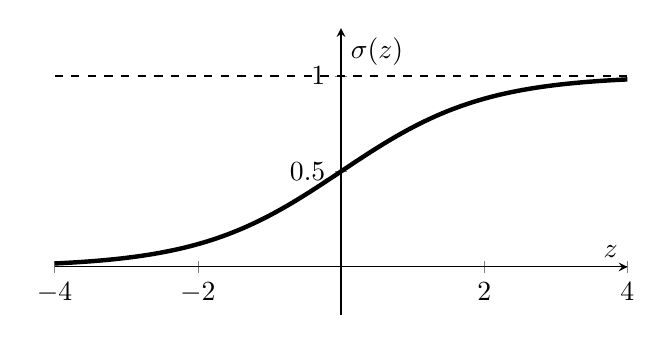
\begin{tikzpicture}
    \begin{axis}[
        axis lines=middle,
        % axis equal image,
        scale only axis,
        width=0.6\textwidth,
        height=0.3\textwidth,
        xmin=-4, xmax=4,
        ymin=-0.25, ymax=1.25,
        xlabel={$z$}, ylabel={$\sigma(z)$},
      ]
      \addplot [domain=-4:4, samples=100, ultra thick] {1/(1+exp(-x))};
      \addplot [domain=-4:4, samples=2, dashed] {1};
      \addplot [domain=-4:4, samples=2, dashed] {0};
    \end{axis}
  \end{tikzpicture}
\end{center}

\question{Convince yourself the output of $\sigma$ is always in the
  interval $(0, 1)$.  Why can't it equal 0 or equal 1?  For what value
  of $z$ does $\sigma(z) = 0.5$?}

\subsection{Linear logistic classifier: examples}

What does an LLC look like?   Let's consider the
simple case where $d = 1$, so our input points simply lie along the
$x$ axis.  Classifiers in this case have dimension $0$, meaning that
they are points.
The plot below shows LLCs for three different parameter
settings: $\sigma(10x + 1)$, $\sigma(-2x + 1)$, and $\sigma(2x - 3).$
\begin{center}
  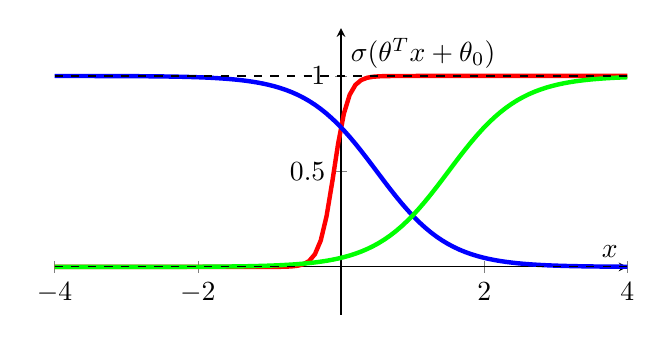
\begin{tikzpicture}
    \begin{axis}[
        axis lines=middle,
        % axis equal image,
        scale only axis,
        width=0.6\textwidth,
        height=0.3\textwidth,
        xmin=-4, xmax=4,
        ymin=-0.25, ymax=1.25,
        xlabel={$x$}, ylabel={$\sigma(\theta^T x + \theta_0)$},
      ]
      \addplot [domain=-4:4, samples=100, ultra thick, red] {1/(1+exp(-(10*x + 1)))};
      \addplot [domain=-4:4, samples=100, ultra thick, blue] {1/(1+exp(-(-2*x
        + 1)))};
      \addplot [domain=-4:4, samples=100, ultra thick, green] {1/(1+exp(-(2*x
        - 3)))};
      \addplot [domain=-4:4, samples=2, dashed] {1};
      \addplot [domain=-4:4, samples=2, dashed] {0};
    \end{axis}
  \end{tikzpicture}
\end{center}
\question{Which plot is which?  What governs the steepness of the
  curve?  What governs the $x$ value where the output is equal to
  0.5?}

But wait!  Remember that the definition of a classifier is that it's a mapping from $\R^d
  \rightarrow \{-1, +1\}$ or to some other discrete set.  So, then, it
seems like an LLC is actually not a classifier!

Given an LLC, with an output value in $(0, 1)$, what should we do if
we are forced to make a prediction in $\{+1, -1\}$?  A default answer
is to predict $+1$ if $\sigma(\theta^T x + \theta_0) > 0.5$ and $-1$
otherwise.  The value $0.5$ is sometimes called a {\em prediction
    threshold}.\index{logistic linear classifier!prediction threshold}

In fact, for different problem settings, we might prefer to pick a
different prediction threshold.  The field of {\em decision theory}
considers how to make this choice.
For example, if the consequences of predicting $+1$ when
the answer should be $-1$ are much worse than the consequences of
predicting $-1$ when the answer should be $+1$, then we might set the
prediction threshold to be greater than $0.5$.

\question{Using a prediction threshold of 0.5, for what values of $x$
  do each of the LLCs shown in the figure above predict $+1$?}

When $d = 2$, then our inputs $x$ lie in a two-dimensional space with
axes $x_1$ and $x_2$, and the output of the LLC is a surface, as shown
below, for $\theta = (1, 1), \theta_0 = 2$.

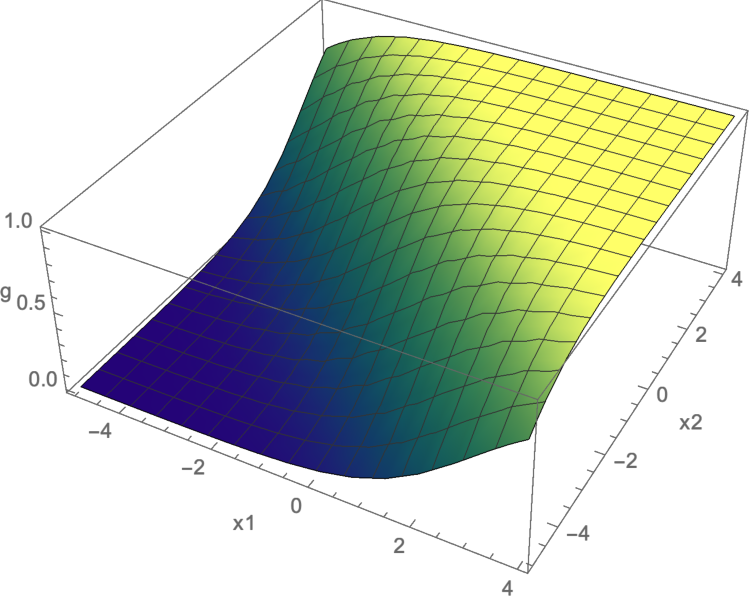
\includegraphics[width=0.7\textwidth]{figures/logreg3d}

\question{Convince yourself that the set of points for which
  $\sigma(\theta^T x + \theta_0) = 0.5$, that is, the ``boundary''
  between positive and negative predictions with prediction threshold
  $0.5$, is a line in $(x_1, x_2)$ space. What particular line is it
  for the case in the figure above?
  How would the plot change for $\theta = (1, 1)$, but now
  with $\theta_0 = -2$? For $\theta = (-1, -1), \theta_0 = 2$?}

%%%%%%%%%%%%%%%%%%%%%%%%%%%%%%%%%%%%%%%%
\subsection{Learning linear logistic classifiers}

\label{logistic}

Optimization is a key approach to solving machine learning
problems; this also applies to learning linear logistic classifiers (LLCs) by
defining an appropriate loss function for optimization.
A first attempt might be to use the simple 0-1 loss function $\mathcal{L}_{01}$
that gives a value of 0 for a correct prediction, and a 1 for an
incorrect prediction. As noted earlier, however, this gives rise
to an objective function that is very difficult to optimize, and so
we pursue another strategy for defining our objective.

For learning LLCs, we'd have a class of hypotheses
whose outputs are in $(0, 1)$, but for which we have training data with $y$
values in $\{+1, -1\}$.  How can we define an appropriate loss
function?  We start by changing our interpretation of the output to be
  {\em the probability that the input should map to output value 1} (we
might also say that this is the probability that the input is in class 1 or
that the input is `positive.')
\question{If $h(x)$ is the probability that $x$ belongs to class $+1$,
  what is the probability that $x$ belongs to the class $-1$, assuming there are only these two classes?}

Intuitively, we would like to have
  {\em low loss if we assign a high probability to the correct class.}
We'll define a loss function, called {\em negative log-likelihood} (NLL)\index{negative log-likelihood},
that does just this.  In  addition, it has the cool property that it
extends nicely to the case where we would like to classify our inputs
into more than two classes.

In order to simplify the description, we assume that (or transform our
data so that) the labels
in the training data are $y \in \{0, 1\}$.
\note{\bf Remember to be sure your $y$
  values have this form if you try to learn an LLC using NLL!}

We would like to pick the parameters of our classifier to maximize the
probability assigned by the LLC to the correct $y$ values, as
specified in the training set.  Letting guess $\ex{g}{i} =
  \sigma(\theta^T\ex{x}{i} + \theta_0)$,
that probability is\note{That crazy huge $\Pi$ represents taking the
  product over a bunch of factors just as huge $\Sigma$ represents
  taking the sum over a bunch of terms.}
\begin{equation*}
  \prod_{i = 1}^n \begin{cases} \ex{g}{i} & \text{if $\ex{y}{i} =
              1$}                               \\ 1 - \ex{g}{i} & \text{otherwise}
  \end{cases}\;\;,
\end{equation*}
under the assumption that our predictions are independent.  This can
be cleverly rewritten, when $\ex{y}{i} \in \{0, 1\}$, as
\begin{equation*}
  \prod_{i = 1}^n {\ex{g}{i}}^{\ex{y}{i}}(1 - \ex{g}{i})^{1 - \ex{y}{i}}\;\;.
\end{equation*}
\question{Be sure you can see why these two expressions are  the
  same.}

The big product above is kind of hard to deal with in practice, though.
So what can we do?
Because the
log function is monotonic, the $\theta, \theta_0$ that maximize the
quantity above will be the same as the $\theta, \theta_0$ that
maximize its log, which is the following:
\begin{equation*}
  \sum_{i = 1}^n  \left( {\ex{y}{i}}\log {\ex{g}{i}} +
  (1 - \ex{y}{i})\log(1 - \ex{g}{i})\right)\;\;.
\end{equation*}
Finally, we can turn the maximization problem above into a minimization problem by taking the negative
of the above expression, and writing in terms of minimizing a loss
\begin{equation*}
  \sum_{i = 1}^n \mathcal{L}_\text{nll}(\ex{g}{i}, \ex{y}{i})
\end{equation*}
where $\mathcal{L}_\text{nll}$ is the {\em negative log-likelihood}
loss function:
\begin{equation*}
  \mathcal{L}_\text{nll}(\text{guess},\text{actual}) =
  -\left(\text{actual}\cdot \log (\text{guess}) + (1 - \text{actual})\cdot\log (1 -
  \text{guess})\right) \;\;.
\end{equation*}
This loss function is also sometimes referred to as the {\em log loss}
or {\em cross entropy}\index{negative log-likelihood!loss function}. \note{You can use any base for the logarithm
  and it won't make any real difference.  If we ask you for numbers,
  use log base $e$.}

{\bf What is the objective function for linear logistic classification?}
We can finally put all these pieces together and develop an objective
function for optimizing regularized negative log-likelihood for a
linear logistic classifier. \note{That's a lot of fancy words!}  In
fact, this process is usually called ``logistic regression,'' so
we'll call our objective $J_\text{lr}$, and define it as
\begin{equation}
  J_\text{lr}(\theta, \theta_0; {\cal D}) =
  \left(\frac{1}{n} \sum_{i=1}^n
  \mathcal{L}_\text{nll}(\sigma(\theta^T \ex{x}{i} + \theta_0), \ex{y}{i})\right) +
  \lambda \norm{\theta}^2\;\;.
  \label{eq:lr_with_reg}
\end{equation}

\question{Consider the case of linearly separable data.   What will
  the $\theta$ values that optimize this objective be like if
  $\lambda = 0$?   What will they be like if $\lambda$ is very big?
  Try to work out an example in one dimension with two data points.}

{\bf What role does regularization play for classifiers?}
This objective function has the same structure as the one we used for
regression, Eq.~\ref{eq:ml_objective_loss}, where the first term (in
parentheses) is the average loss, and the second term is for regularization.
Regularization is needed for building classifiers that can generalize
well (just as was the case for regression).  The parameter $\lambda$ governs
the trade-off between the two terms as illustrated in the following example.


Suppose we wish to obtain a linear logistic classifier for this one-dimensional dataset:

\centerline{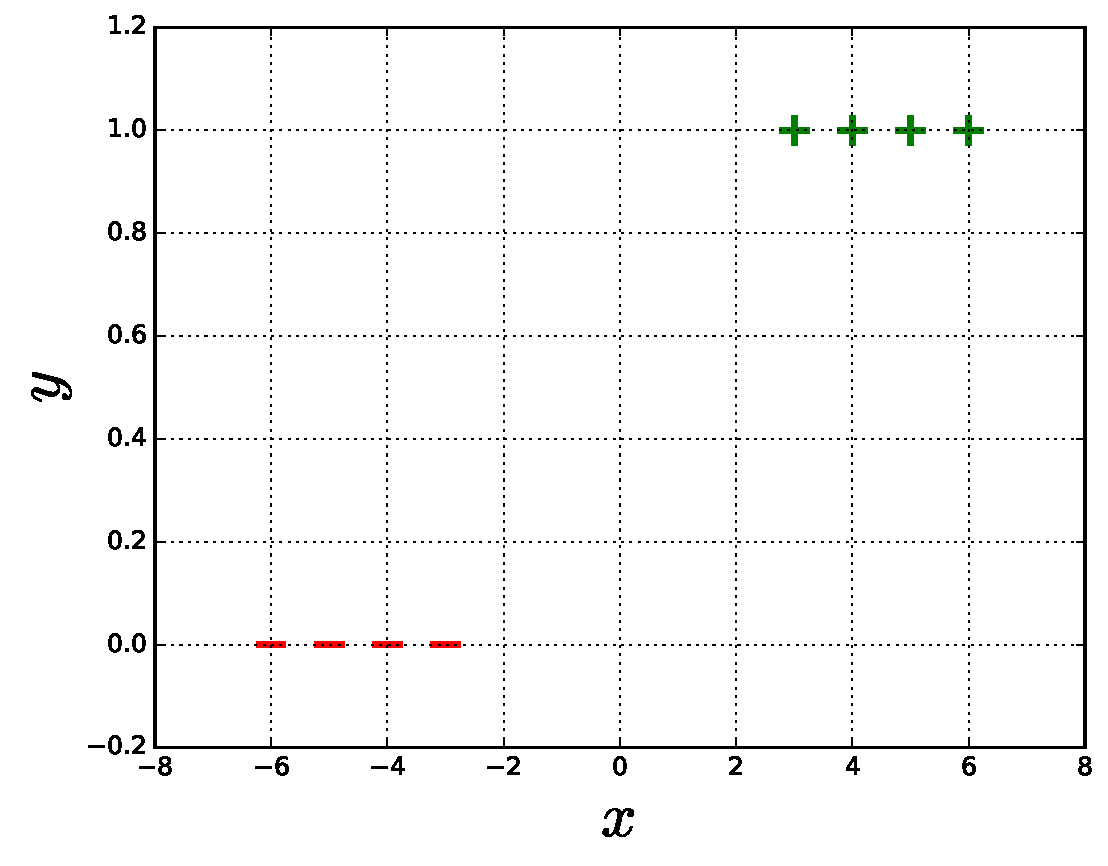
\includegraphics[width=0.45\textwidth]{figures/linear_logistic_classifier_and_regularization_data}}

%
\noindent
Clearly, this can be fit very nicely by a hypothesis
$h(x)=\sigma(\theta x)$, but what is the best value for $\theta$?
Evidently, when there is no regularization ($\lambda=0$), the objective function $J_{lr}(\theta)$ will approach zero for large
values of $\theta$, as shown in the plot on the left, below.
However, would the best hypothesis really have an infinite (or very
large) value for $\theta$?  Such a hypothesis would suggest that the
data indicate strong certainty that a sharp transition between $y=0$
and $y=1$ occurs exactly at $x=0$, despite the actual data having a wide
gap around $x=0$.
%
\centerline{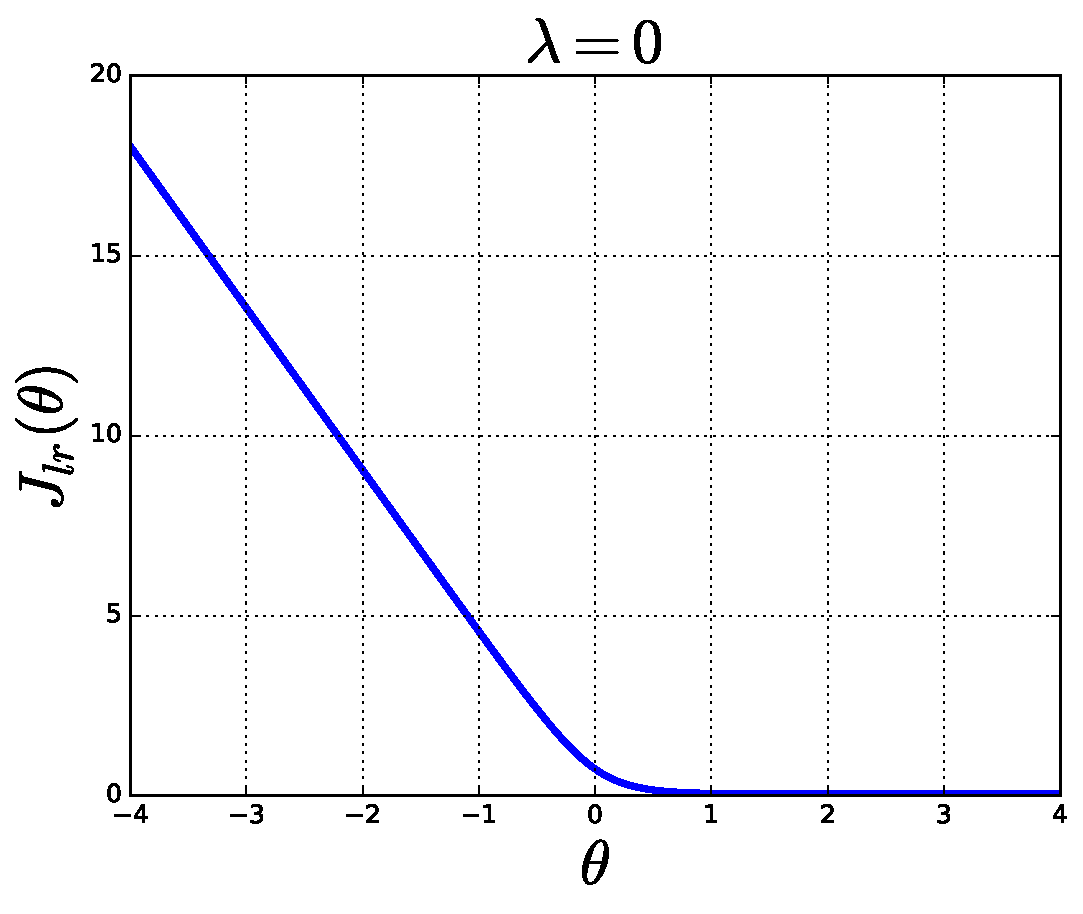
\includegraphics[width=0.45\textwidth]{figures/linear_logistic_classifier_and_regularization_objective_noreg}
  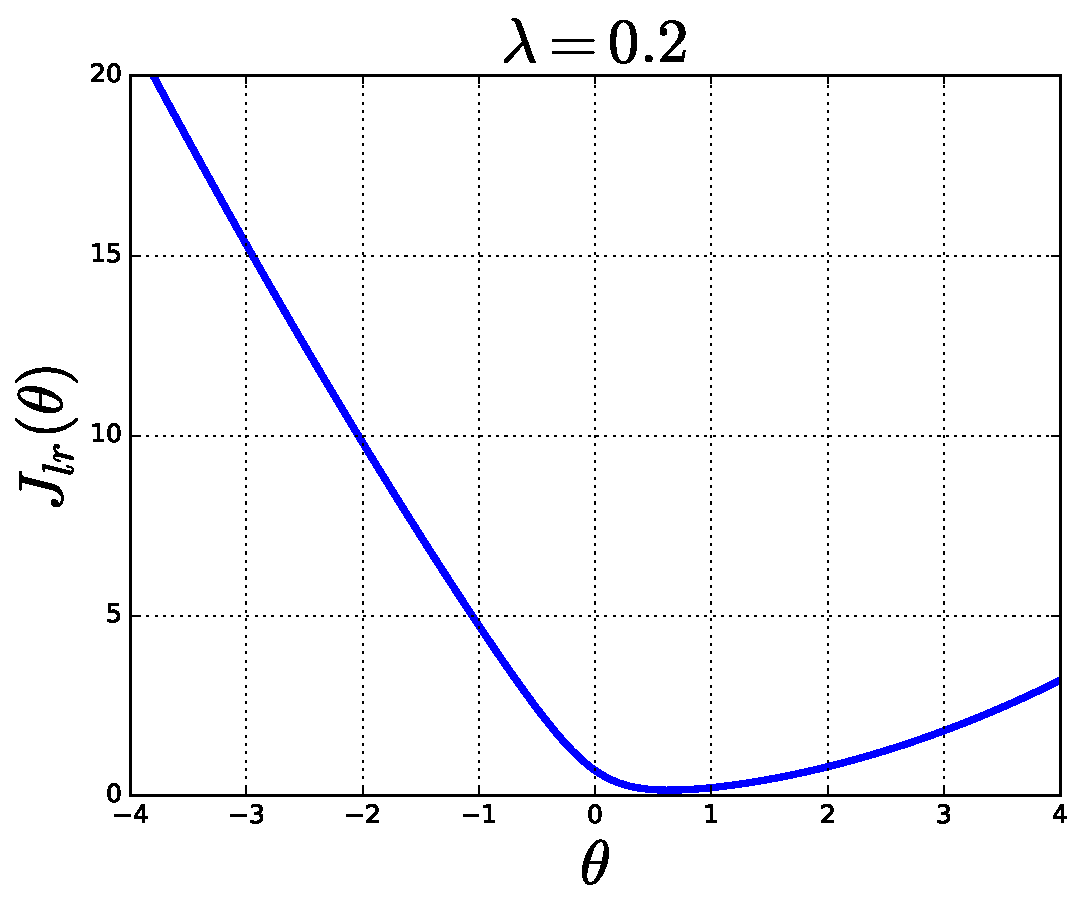
\includegraphics[width=0.45\textwidth]{figures/linear_logistic_classifier_and_regularization_objective_withreg}
}
%

\question{Be sure this makes sense.  When the $\theta$ values are
  very large, what does the sigmoid curve look like?  Why do we say
  that it has a strong certainty in that case?
}

In absence of other beliefs about the solution, we might prefer that
our linear logistic classifier not be overly certain about its
predictions, and so we might prefer a smaller $\theta$ over a large
$\theta.$ By not being overconfident, we might expect a somewhat
smaller $\theta$ to perform better on future examples drawn from this
same distribution.\note{To refresh on some vocabulary, we say that in
  this example, a very large $\theta$ would be {\em overfit} to the
  training data.}  This preference can be realized using a nonzero
value of the regularization trade-off parameter, as illustrated in the
plot on the right, above, with $\lambda=0.2$.

Another nice way of thinking about regularization is that we
would like to prevent our hypothesis from being too dependent on the
particular training data that we were given: we would like for it to
be the case that if the training data were changed slightly, the
hypothesis would not change by much.


% Hypothesis $h_1$ has zero training loss, but is
% very complicated.  Hypothesis $h_2$ mis-classifies two points, but is
% very simple.  In absence of other beliefs about the solution, it is
% often better to prefer that the solution be ``simpler,'' and so we
% might prefer $h_2$ over $h_1$, expecting it to perform better on
% future examples drawn from this same distribution.  \note{To establish
%   some vocabulary, we say that $h_1$ is {\em overfit} to the training
%   data.}  
% 
% \begin{center}
% \begin{tikzpicture}
%   \draw [->] (-4,0) -- (4,0);
%   \draw [->] (0,-4) -- (0,4);
%   \draw[red,thick] (-2.5,-3) .. controls (-4,1) and (-3.8,1.2) .. (-2.4,-.5)
%     .. controls (-2,-1) .. (-1,-1) .. controls (-.5,-1) ..  (.5,-2)
%     .. controls (.65, -2.1) .. (.7,-1.8) .. controls (.7,-1.5)
%     ..  (.6,-1.2) .. controls (.2,-.4) .. (1.2, -.3)
%     .. controls (1.6,-.2) .. (1,4);
% 
%   \foreach \Point in {(-3.4, .3), (2.5, .2), (-1.5,-2), (-1,-3),(.7,-.7),
%     (3, -2), (2.5, -3.2), (-.7,-1.2), (0.1,-1.8), (1.5, -1.5)}{
%     \draw \Point circle[radius=2pt];
%   }
%   \foreach \Point in {(.5,-1.7),(-.2,.3),(-2.8,.2),(-2.4,-.3),(-1,2.7),
%     (-1.5, 2), (-1.6, .9), (-3.8,-1), (-3.5,1.2),(.5, 1.2)}{
%   \fill \Point circle[radius=2pt];
%   }
%   \draw[blue, thick] (-3.5,-1.8) -- (3.5,1.3);
%   \node[right,blue] at (3.5,1.3) {$h_2$};
%   \node[below,right,red] at (1,4) {$h_1$};
% 
% \end{tikzpicture}
% \end{center}



\section{Gradient descent for logistic regression}

\label{sec-gd_lrr}

% Recall  that choosing a loss function is the
% first step in formulating a machine-learning problem as an
% optimization problem, and for regression we studied the mean square
% loss, Eq.~\ref{eq:reg_mse}, which captures loss as
% $({\rm guess} - {\rm actual})^2$.  The derivative of this,
% Eq.~\ref{eq:reg_gd_deriv}, was used previously to obtain an
% analytical solution to the linear regression problem.  Gradient
% descent could also be applied to numerically compute a solution, using
% the update rule
% \begin{equation}
%   \ex{\Theta}{t} = \ex{\Theta}{t-1} - \eta \frac{2}{n} \sum_{i=1}^{n} \left( \left[ \ex{\Theta}{t-1}\right]^T x^{(i)} - y^{(i)} \right) x^{(i)}
% \,.
% \end{equation}
% {~\hfill ~\note{Beware double superscripts!  $\left[ \Theta \right]^T$ is the transpose of the vector $\Theta$}}

% But what happens when the models are nonlinear, and the loss function
% is more complicated than being merely mean squared error?  Analytical
% solutions rarely exist for more complex situations, but gradient
% descent can still be applied, especially when the derivatives of the
% loss function can be computed analytically.  We will see this by
% applying gradient descent to $J_\text{lr}$, the logistic regression
% objective. 


% For classification, we
% are interested in the {\em negative log-likelihood} loss function
% (written more compactly as):
% \begin{equation}
%   \mathcal{L}_\text{nll}(\ex{g}{i}, \ex{y}{i})  = - {\ex{y}{i}}\log {\ex{g}{i}} - (1 - \ex{y}{i})\log(1 - \ex{g}{i})
% \;\;
% \end{equation}
% where the correct values $\ex{y}{i}$ are now assumed to be either $0$
% or $1$, and $\ex{g}{i}$ are our guesses.  These guesses are computed
% using the model parameters $\Theta = (\theta, \theta_0)$ as
% \begin{equation}
%   \ex{g}{i} = \sigma(\theta^T \ex{x}{i} + \theta_0)
% \,,
% \end{equation}
% where $\sigma$ is some {\em nonlinear} function which maps $\R$ to
% real numbers in the range $0$ to $1$ (inclusive of the endpoints).
% In what follows, we use the function $\sigma(z) = \frac{1}{1+e^{-z}}$. (See the next chapter for
% more intuition about why.)
% Combining this with a ridge regularization term, we obtain this
% ``logistic regression'' objective function:
% \begin{equation}
%   J_\text{lr}(\theta,\theta_0) = \frac{1}{n}\sum_{i=1}^n
%                                  \mathcal{L}_\text{nll}
%                                  (\ex{g}{i}, \ex{y}{i}) + \frac{\lambda}{2}\norm{\theta}^2
%                                \end{equation}

Now that we have a hypothesis class (LLC) and a loss function (NLL),
we need to take some data and find parameters!
Sadly, there is no lovely analytical solution like the one we obtained
for regression, in Section~\ref{sec-ridge_regression}.  Good thing we
studied gradient descent!  We can perform gradient descent on the
$J_{lr}$ objective, as we'll see next.  We can also apply stochastic
gradient descent to this problem.

Luckily, $J_{lr}$ has enough nice properties that gradient descent and
stochastic gradient descent should generally ``work''. We'll soon see
some more challenging optimization problems though -- in the
context of neural networks, in Section~\ref{sec-make_nn_work}.

First we need derivatives with respect to both $\theta_0$ (the scalar
component) and $\theta$ (the vector component) of $\Theta$.
Explicitly, they are: \note{Some passing familiarity with matrix
  derivatives is helpful here.  A foolproof way of computing them is
  to compute partial derivative of $J$ with respect to each component
  $\theta_i$ of $\theta$.}
\begin{align*}
  \nabla_\theta J_\text{lr}(\theta, \theta_0)                      & =  \frac{1}{n}\sum_{i=1}^n
  \left(\ex{g}{i} -
  \ex{y}{i}\right) \ex{x}{i}
  + 2\lambda\theta                                                                              \\
  \frac{\partial J_\text{lr}(\theta, \theta_0)}{\partial \theta_0} & =
  \frac{1}{n}\sum_{i=1}^n
  \left(\ex{g}{i} -
  \ex{y}{i} \right) \;\;.
\end{align*}
Note that $\nabla_\theta J_\text{lr}$ will be of shape $d \times 1$ and
$\frac{\partial J_\text{lr}}{\partial \theta_0}$ will be a scalar since
we have separated $\theta_0$ from $\theta$ here.
\question{Convince yourself that the dimensions of all these
  quantities are correct, under the assumption that $\theta$ is $d
    \times 1$. 
}

\question{Compute $\nabla_\theta \norm{\theta}^2$ by finding the
  vector of partial derivatives $(\partial \norm{\theta}^2 / \partial
    \theta_1, \ldots, \partial \norm{\theta}^2 / \partial
    \theta_d)$. What is the shape of $\nabla_\theta \norm{\theta}^2$?
}

\question{Compute $\nabla_\theta \mathcal{L}_\text{nll}(
  \sigma(\theta^T x + \theta_0), y)$ by finding the
vector of partial derivatives $(\partial \mathcal{L}_\text{nll}(
  \sigma(\theta^T x + \theta_0), y)/ \partial \theta_1, \ldots,
  \partial \mathcal{L}_\text{nll}(
  \sigma(\theta^T x + \theta_0), y) / \partial
  \theta_d)$.
  }

  \question{Use these last two results to verify our derivation above.}

  Putting everything together, our gradient descent algorithm for logistic
  regression becomes:\index{gradient descent!applied to logistic regression}
  \begin{codebox}
    \Procname{$\proc{LR-Gradient-Descent}(\theta_{\it init}, \theta_{0
          {\it init}},\eta,\epsilon)$}
    \li $\theta^{(0)} \gets \theta_{\it init}$
    \li $\theta_0^{(0)} \gets \theta_{0 {\it init}}$
    \li $t \gets 0$
    \li \Repeat
    \li   $t \gets t+1$
    \li   $\theta^{(t)} = \theta^{(t-1)} - \eta\left(\frac{1}{n}\sum_{i=1}^n
      \left(\sigma\left({\ex{\theta}{t-1}}^T \ex{x}{i} + \ex{\theta_0}{t-1}\right) -
        \ex{y}{i}\right) \ex{x}{i}
      + 2\lambda\ex{\theta}{t-1}
      \right)$
    \li   $\theta_0^{(t)} = \theta_0^{(t-1)} - \eta\left(\frac{1}{n}\sum_{i=1}^n
      \left(\sigma\left({\ex{\theta}{t-1}}^T \ex{x}{i} + \ex{\theta_0}{t-1}\right) -
        \ex{y}{i} \right)
      \right)$
    \li \Until $\left| J_{\text{lr}}(\theta^{(t)},\theta_0^{(t)}) - J_{\text{lr}}(\theta^{(t-1)},
      \theta_0^{(t-1)}) \right| <\epsilon$
    \li \Return $\theta^{(t)},\theta_0^{(t)}$
  \end{codebox}


  Logistic regression, implemented using batch or stochastic gradient
  descent, is a useful and fundamental machine learning technique. We
  will also see later that it corresponds to a one-layer neural network
  with a sigmoidal activation function, and so is an important step
  toward understanding neural networks.

  \subsection{Convexity of the NLL Loss Function}

  Much like the squared-error loss function that we saw for linear regression,
  the NLL loss function for linear logistic regression is a convex function.
  This means that running gradient descent with a reasonable set of hyperparameters
  will converge arbitrarily close to the minimum of the objective function.

  We will use the following facts to demonstrate that the NLL loss function is a convex function:
  \begin{itemize}
    \item if the derivative of a function of a scalar argument is monotonically increasing, then it is a convex function,
    \item the sum of convex functions is also convex,
    \item a convex function of an affine function is a convex function.
  \end{itemize}
  Let $z=\theta^T x + \theta_0$; $z$ is an affine function of $\theta$ and $\theta_0$.
  It therefore suffices to show that the functions $f_1(z) = - \log (\sigma(z))$ and
$f_2 (z) = -\log (1 - \sigma(z))$ are convex with respect to $z$.

  First, we can see that since,
  \begin{align*}
    \frac{d}{dz} f_1(z) & = \frac{d}{dz} \left[ -\log (1/(1 + \exp (-z))) \right], \\
                        & = \frac{d}{dz} \left[ \log (1 + \exp (-z)) \right],      \\
                        & = - \exp (-z) / (1 + \exp (-z)),                         \\
                        & = -1 + \sigma(z),
  \end{align*}
  the derivative of the function $f_1 (z)$ is a monotonically increasing function and
  therefore $f_1$ is a convex function.

  Second, we can see that since,
  \begin{align*}
    \frac{d}{dz} f_2(z) & = \frac{d}{dz} \left[ -\log (\exp(-z)/(1 + \exp (-z))) \right], \\
                        & = \frac{d}{dz} \left[ \log (1 + \exp (-z)) + z \right],         \\
                        & = \sigma(z),
  \end{align*}
  the derivative of the function $f_2(z)$ is also monotonically increasing and
  therefore $f_2$ is a convex function.

  \section{Handling multiple classes}

  So far, we have focused on the {\em binary} classification case, with
  only two possible classes.  But what can we do if we have multiple
  possible classes (e.g., we want to predict the genre of a movie)?
  There are two basic strategies:
  \begin{itemize}
    \item Train multiple binary classifiers using different subsets of
          our data and combine their outputs to make a class prediction.
    \item Directly train a multi-class classifier using a hypothesis
          class that is a generalization of logistic regression, using a
            {\em one-hot} output encoding and NLL loss.
  \end{itemize}

  %% We will explore both methods below, but the method based on NLL is
  %% in wider use, especially in the context of neural networks.

  %% \subsection{Reducing multi-class to binary}

  %% There are two standard strategies for reducing multi-class
  %% classification to binary classification.\index{classification!multi-class classification}

  %% In the {\em one versus all} (OVA) strategy\index{classification!multi-class classification!one versus all}, we will train $K$
  %% different binary classifiers.  To train classifier $k$, we
  %% \begin{itemize}
  %% \item Create a training set $\data_k$ in which all $\ex{x}{i} \in D$
  %%   for which $\ex{y}{i} = k$ are assigned label $+1$ and all other
  %%   $\ex{x}{i}$ are assigned label $-1$.
  %% \item Use logistic regression (or any other classifier-learning
  %%   method) to obtain a hypothesis $h_k$ by training on $\data_k$.
  %%   \end{itemize}
  %% Then, we create a new multi-class hypothesis 
  %%   \[h(x) = \argmax{k} h_k(x)\;\;,\]
  %%   that predicts the class $k$ to which this example was
  %%   assigned with highest confidence by the individual hypotheses.

  %%   In the {\em one versus one} (OVO) strategy\index{classification!multi-class classification!one versus one}, we will train
  %% $K(K-1)/2$ classifiers, one for each unique pair $j, k$ (where $j \not= k$) of classes.  To
  %% train classifier $j, k$, we
  %% \begin{itemize}
  %% \item Create a training set $\data_{jk}$ in which all $\ex{x}{i} \in D$
  %%   for which $\ex{y}{i} = j$ are assigned label $+1$ and
  %%  all $\ex{x}{i} \in D$ for which $\ex{y}{i} = k$ are assigned label $-1$.
  %% \item Use logistic regression (or any other classifier-learning
  %%   method) to obtain hypotheses $h_{jk}$ by training on $\data_{jk}$.
  %% \end{itemize}
  %% Then, given a new input $x$, we feed it into each of the classifiers $h_{jk}$
  %% and obtain a {\em binary} decision about whether it is more likely to
  %% be in class $j$ or class $k$.  We generate as output the class that is
  %% selected as the ``winner'' in the majority of the cases.

  %% \subsection{Multi-class classification and log likelihood}

  The method based on NLL is in wider use, especially in the context of
  neural networks, and is explored here.
  In the following, we will assume that we have a data set $\data$ in
  which the inputs
$\ex{x}{i} \in R^d$ but the outputs $\ex{y}{i}$ are drawn from a set
  of $K$ classes $\{c_1, \ldots, c_K\}$.
  Next, we extend the idea of NLL directly to multi-class
  classification\index{negative log-likelihood!multi-class
    classification} with $K$ classes, where the training label is
  represented with what is called a {\em one-hot} vector
$y=\begin{bmatrix} y_1, \ldots, y_K \end{bmatrix}^T$, where $y_k=1$ if
  the example is of class $k$ and $y_k = 0$ otherwise.
  Now, we have a problem of mapping an input $\ex{x}{i}$ that is in
$\R^d$ into a $K$-dimensional output.  Furthermore, we would like this
  output to be interpretable as a discrete probability distribution over
  the possible classes, which means the elements of the output vector have to
  be {\em non-negative} (greater than or equal to 0) and sum to 1.

  We will do this in two steps.  First, we will map our input
$\ex{x}{i}$ into a vector value $\ex{z}{i} \in \R^K$ by letting $\theta$ be a
  whole $d \times K$ {\em matrix} of parameters, and $\theta_0$ be a $K
\times 1$ vector, so that
  \[z = \theta^T x + \theta_0\;\;.\]
  \note{Let's check dimensions!  $\theta^T$ is $K \times d$ and $x$ is
    $d \times 1$, and $\theta_0$ is $K \times 1$, so $z$ is $K \times
      1$ and we're good!}
  Next, we have to extend our use of the sigmoid function to the
  multi-dimensional {\em softmax} function, that takes
  a whole vector $z \in \R^K$ and generates
  \[g = \textit{softmax}(z) =
    \begin{bmatrix}
      \exp(z_1) / \sum_{i} \exp(z_i) \\
      \vdots                         \\
      \exp(z_K) / \sum_{i} \exp(z_i)
    \end{bmatrix}\;\;.\]
  which can be interpreted as a probability distribution over $K$ items. To make the final prediction of the class label, we can then look at $g,$ find the most likely probability over these $K$ entries in $g,$ (i.e. find the largest entry in $g,$) and return the corresponding index as the ``one-hot'' element of $1$ in our prediction.

  \question{Convince yourself that the vector of $g$ values will be
    non-negative and sum to 1.}

  Putting these steps together, our hypotheses will be
  \[h(x; \theta, \theta_0) = \textit{softmax}(\theta^T x + \theta_0)\;\;.\]

  Now, we retain the goal of maximizing the probability that our
  hypothesis assigns to the correct output $y_k$ for each input $x$.  We
  can write this probability, letting $g$ stand for our ``guess'', $h(x)$, for a
  single example $(x, y)$ as $\prod_{k = 1}^K g_k^{y_k}$.
  \question{How many elements that are not equal to 1 will there be in this product?}

  The negative log of the probability that we are making a correct guess is, then, for {\em one-hot} vector $y$ and {\em probability distribution}
  vector $g$,
$$\mathcal{L}_\text{nllm}(\text{g},\text{y}) =
  - \sum_{k=1}^K \text{y}_k \cdot \log(\text{g}_k) \;\;.$$
We'll call this {\sc nllm} for {\em negative log likelihood
    multiclass.} It is also worth noting that the NLLM loss function is also convex; however, we will omit the proof.
\question{Be sure you see that is $\mathcal{L}_\text{nllm}$ is minimized when the guess assigns high probability to the true class.}
\question{Show that $\mathcal{L}_\text{nllm}$ for $K = 2$ is the same as
  $\mathcal{L}_\text{nll}$. }

\section{Prediction accuracy and validation}

In order to formulate classification with a smooth objective function
that we can optimize robustly using gradient descent, we changed the
output from discrete classes to probability values and the loss
function from 0-1 loss to NLL.
However, when time comes to actually make a prediction we usually have
to make a hard choice:  buy stock in Acme or not?  And, we get
rewarded if we guessed right, independent of how sure or not we were
when we made the guess.

The performance of a classifier is often characterized by its {\em
    accuracy}, which is the percentage of a data set that it predicts
correctly in the case of 0-1 loss. We can see that accuracy of hypothesis $h$ on data $\data$
is the fraction of the data set that does not incur any loss:
\[A(h; \data) = 1 - \frac{1}{n}\sum_{i=1}^n\mathcal{L}_{01}(\ex{g}{i}, \ex{y}{i})\;\;,\]
where $\ex{g}{i}$ is the final guess for one class or the other
that we make from $h(\ex{x}{i})$, e.g., after thresholding.
It's noteworthy here that we use a different loss function for optimization
than for evaluation. This is a compromise we make for computational
ease and efficiency.



%%% Local Variables:
%%% mode: latex
%%% TeX-master: "top"
%%% End:

